% This is samplepaper.tex, a sample chapter demonstrating the
% LLNCS macro package for Springer Computer Science proceedings;
% Version 2.20 of 2017/10/04
%
\documentclass[runningheads]{llncs}
%
\usepackage[hyphens]{url}
\usepackage[pdftex]{graphicx}
\usepackage{amsmath,amssymb}
%\usepackage{accents}
%\usepackage{amsthm}
\usepackage{array}
\usepackage{bm}
\usepackage{color}
\usepackage{etex}
\usepackage{extramacros}
%\usepackage{fullpage}
\usepackage{graphicx}
\usepackage{hyperref}
\usepackage{mathtools}
\usepackage{stackrel}


%\usepackage{graphicx}
% Used for displaying a sample figure. If possible, figure files should
% be included in EPS format.
%
% If you use the hyperref package, please uncomment the following line
% to display URLs in blue roman font according to Springer's eBook style:
\renewcommand\UrlFont{\color{blue}\rmfamily}

\begin{document}
%
\title{Gradient flow to the Kantorovich coupling\thanks{The author is
    supported by de Castro Statistics and Collegio Carlo Alberto.}}
%
%\titlerunning{Abbreviated paper title}
% If the paper title is too long for the running head, you can set
% an abbreviated paper title here
%
\author{Giovanni Pistone\inst{1}\orcidID{0000-0003-2841-788X}}
%
\authorrunning{G. Pistone}
% First names are abbreviated in the running head.
% If there are more than two authors, 'et al.' is used.
%
\institute{De Castro Statistics, Collegio Carlo Alberto, Piazza
  Arbarello 8, 10122 Torino, Italy \\
  \email{giovanni.pistone@carloalberto.org}\\
  \url{https://www.giannidi orestino.it}}
%
\maketitle              % typeset the header of the contribution
%
\begin{abstract}
We discuss the gradient flow problem for the Kantorovich distance on a
finite sample space.
\keywords{Gradient flow \and Kantorovich optimal transport \and
  Statistical bundle.}
\end{abstract}
%
%
%
\section{Introduction}
Consider a product finite sample space
$\Omega=\Omega_1 \times \Omega_2$ and marginal mappings
$X \colon \Omega \to \Omega_1$, $Y \colon \Omega \to \Omega_2$. If
$\gamma$ is a probability function on $\Omega$, we denote by
$\gamma_1$ and $\gamma_2$ the image probability functions on
$\Omega_1$ and $\Omega_2$, respectively. We denote by $L(\Omega)$,
$L(\Omega_1)$ and $L(\Omega_2)$ the spaces of real random variables
and by $L_0(\gamma)$, $L_0(\gamma_1)$ and $L_0(\gamma_2)$ the spaces
of random variables which are centered for the given probability
function.

We use the non-parametric version of Information Geometry as described
in the tutorial \cite{pistone:2020-NPCS}. In this setup,
$\Delta^\circ(\Omega)$ is the interior of the probability simplex and
$S = S\Delta^\circ(\Omega)$ is the \emph{statistical bundle}, that is, the
set of all couples $(\gamma,u)$ with $\gamma \in \Delta^\circ(\Omega)$
and $u$ a random variable such that $\expectat \mu u=0$. For each
smooth curve $t \mapsto \gamma(t) \in \Delta^\circ(\Omega)$ the
\emph{velocity} $\velocity \gamma(t) = \derivby t \log \gamma(t)$ is
characterised by
\begin{equation}
  \label{eq:1}
  \derivby t \expectat {\gamma(t)} u = \scalarat {\gamma(t)} {\velocity
  \gamma(t)} u \ .
\end{equation}

On a sub-manifold, each fiber $S_\gamma$ of the
statistical bundle splits to define a proper sub-statistical bundle. 

We are interested in the sub-manifold of tranport plans. Let be given
$\mu_1 \in \Delta^\circ(\Omega_1)$ and $\mu_2 \in
\Delta^\circ(\Omega_2)$. The \emph{transport plan model} with margins $\mu_1$ and $\mu_2$ is the statistical model
%
  \begin{equation*}
    \Gamma(\mu_1,\mu_2) = \setof{\gamma \in \Delta(\Omega)}{X_\# \gamma = \mu_1, Y_\# \gamma = \mu_2} \ ,
  \end{equation*}
%
where $\Omega=\Omega_1 \times \Omega_2$. The \emph{open} transport plan is 
%
  \begin{equation*}
    \Gamma^\circ(\mu_1,\mu_2) = \setof{\gamma \in \Delta^\circ(\Omega)}{X_\# \gamma = \mu_1, Y_\# \gamma = \mu_2} \ .
  \end{equation*}
  %

  Let $t \mapsto \gamma(t)$ be a smooth curve in the open transport
  plan. Equation \eqref{eq:1} with $u = f(X)$ gives
  \begin{equation*}
  0 = \derivby t \expectat {\mu_1} f =  \derivby t \expectat
  {\gamma(t)} {f(X)} = \scalarat {\gamma(t)} {\velocity \gamma(t)}
  {f(X)} = \scalarat {\mu_1} {{\velocity \gamma(t)}_1} f \ , 
  \end{equation*}
with ${\velocity \gamma(t)}_1(X) = \condexpectat {\gamma(t)} {\velocity
  \gamma(t)} X$. Similarly for the other margin.

Let us discuss more in detail the relevant splitting in the language
of statistical ANOVA. Let $\gamma$ be
a probability function on $\Omega$. The linear subspaces of the space
of random variables $L(\Omega)$ which describe, respectively, the
$\gamma$-grand-mean, the two \emph{$\gamma$-marginal effects}, and
the \emph{$\gamma$-interactions}, are
%
\begin{equation}\label{eq:ANOVA-spaces}
\begin{aligned}
  L_0(\gamma) &\sim \reals, \\
  L_1(\gamma) &= \setof{f\circ X}{f \in L_0(\gamma_1)},\\
  L_2(\gamma) &= \setof{f\circ Y}{f \in L_0(\gamma_2)},\\
  L_{12}(\gamma) &= (L_0(\gamma) + L_1(\gamma) + L_2(\gamma))^\perp,
\end{aligned}
\end{equation}
%
where orthogonality is computed in the $\gamma$ weight, that is in the scalar product
%%
\begin{equation*}
  (u,v) \mapsto \scalarat \gamma u v = \sum_{\omega\in\Omega}u(\omega)v(\omega)
  \gamma(\omega)\end{equation*}

Each element of the space $L_0(\gamma) + L_1(\gamma) + L_2(\gamma)$
has the form $u = u_0 + f_1(X) + f_2(Y)$, where
$u_0 = \expectat \gamma u$ and $f_1,f_2$ are uniquely defined. More
precisely, we have the following.

\paragraph{1.} \textit{There exist a splitting
%
\begin{equation*}
%
  L(\gamma)) = \reals \oplus \left(L_1(\gamma) + L_2(\gamma)\right) \oplus L_{12}(\gamma) \ . 
\end{equation*}
%
Namely, the splitting of each $u \in L(\gamma)$ is
%
\begin{equation}
 \label{eq:ANOVA}
 u = u_0 + u_1 + u_2 + u_{12} \ ,
\end{equation}
%
where $u_0=\expectat \gamma u$ and $u_1+u_2$ is the
$\gamma$-orthogonal projection of $u$ unto
$L_1(\gamma) + L_2(\gamma)$.}

Each couple of spaces in Eq. \eqref{eq:ANOVA-spaces} has trivial intersection $\set{0}$, hence the splitting of $f \in L(\Omega)$ into $f = f_0 + f_1 + f_2 + f_{1,2}$, with $f_0 \in \reals$, $f_1 \in L_1(\gamma)$, $f_2 \in L_2(\gamma)$, $f_{12} \in L_{12}(\gamma)$ is unique. As $\expectat \gamma f = f_0$ and $L_0(\gamma)$ is orthogonal to $L_1(\gamma)+L_2(\gamma)$, then $f_{12}$ is the orthogonal projection of $f - \expectat \gamma f$ unto $(L_1(\gamma)+L_2(\gamma))^\perp$, while $f_1(\gamma)+f_2(\gamma)$ is the orthogonal projection of $f$ onto $L_1(\gamma)+L_2(\gamma)$.

\paragraph{2.}\textit{The terms $u_1$ and $u_2$ in Eq. \eqref{eq:ANOVA} are characterized by the equations
%
\begin{equation}
\label{eq:projetion}
  \begin{aligned}
    \condexpectat \gamma {(u - u_0)} X u_1 + \condexpectat \gamma {(u-u_0)u_2} X &= 0 \ , \\
    \condexpectat \gamma {(u - u_0)u_1} Y + \condexpectat \gamma {(u-u_0)} Y u_2 &= 0 \ .
  \end{aligned}
%
\end{equation}}

By definition, $(f - f_0) - (f_1 + f_2)$ is $\gamma$-orthogonal to each $g_1+g_2 \in L_1(\gamma)\oplus L_2(\gamma)$ i.e., to each $g_1 \in L_1(\gamma)$ and each $g_2 \in L_2(\gamma)$. The orthogonal projection in such a case is the conditional expectation,
%
  \begin{align*}
    0 &= \condexpectat \gamma {(f-f_0) - (f_1+f_2)}{X}  \ , \\
   0 &= \condexpectat \gamma {(f-f_0) - (f_1+f_2)}{Y} \ .
  \end{align*}
  %

Expressing the conditional expectations with respect to the uniform distribution,
%
  \begin{align*}
    0 &= \condexpectat 0 {\gamma[(f-f_0) - (f_1+f_2)]}{X} \ , \\
   0 &= \condexpectat 0 {\gamma[(f-f_0) - (f_1+f_2)]}{Y} \ ,
  \end{align*}
  % 
that is
%
  \begin{align*}
  \condexpectat 0 {\gamma(f-f_0)} X =  \condexpectat 0 {\gamma} X f_1 + \condexpectat 0 {\gamma f_2} X \ , \\
    \condexpectat 0 {\gamma(f-f_0)} Y =  \condexpectat 0 {\gamma f_1} X  + \condexpectat 0 {\gamma} Y f_2\ .
  \end{align*}
  % 

The ANOVA decomposition proves the existence of the splitting and suggests a computational tool. Assume zero mean, $f_0=0$. The following $(n_1+n_2)\times(n_1+n_2)$ linear system holds:
%
\begin{equation*}
\begin{cases}
  \sum_{y \in \Omega_2} \gamma(x,y)f(x,y) &= \gamma_1(x) f_1(x) + \sum_{y \in \Omega_2} \gamma(x,y) f_2(y) , \quad x \in \Omega_1 \\
  \sum_{x \in \Omega_1} \gamma(x,y)f(x,y) &= \sum_{x \in \Omega_1} \gamma(x,y) f_1(x)  + \gamma_2(y)f_2(y) , \quad y \in \Omega_2
\end{cases}
\end{equation*}
%

Equivalently, using the conditional probabilities $\gamma_{2|1}(y|x) \gamma_1(x) = \gamma_{1|2}(x|y) \gamma_2(y) = \gamma(x,y)$, $x \in \Omega_1$ and $y \in \Omega_2$,
%
\begin{equation*}
\begin{cases}
  \sum_{y \in \Omega_2} \gamma_{2|1}(y|x)f(x,y) &= f_1(x) + \sum_{y \in \Omega_2} \gamma_{2|1}(y|x) f_2(y) , \quad x \in \Omega_1 \\
  \sum_{x \in \Omega_1} \gamma_{1|2}(x|y)f(x,y) &= \sum_{x \in \Omega_1} \gamma_{1|2}(x|y) f_1(x)  + f_2(y) , \quad y \in \Omega_2
\end{cases}
\end{equation*}
%

We write the previous system in matrix form with blocks $\Gamma_{2|1} = [\gamma_{2|1}(y|x)]_{x \in \Omega_1, y \in \Omega_2} \in \reals^{n_1 \times n_2}$ and $\Gamma_{1|2} = [\gamma_{1|2}(x|y)]_{x \in \Omega_1, y \in \Omega_2} \in \reals^{n_1 \times n_2}$, $\bm f_1 = (f_1(x) | x \in \Omega_1)$ and $\bm f_2 = (f_2(x) | x \in \Omega_2)$, $\bm f_{2|1} = (\sum_{y \in \Omega_2} f(x,y)\gamma_{2|1}(y|x) | x \in \Omega_1)$ and $\bm f_{1|2} = (\sum_{x\in\Omega_1} f(x,y)\gamma_{1|2}(x|y) | x \in \Omega_2)$, as 

\begin{equation}
\label{eq:block}
  \begin{bmatrix}
    I_{n_1} & \Gamma_{2|1} \\ \Gamma_{1|2}^T & I_{n_2}
  \end{bmatrix}
  \begin{bmatrix}
    \bm f_1 \\ \bm f_2
  \end{bmatrix}
=
\begin{bmatrix}
  \bm f_{2|1} \\ \bm f_{1|2}
\end{bmatrix}
\end{equation}

The block matrix is not globally invertible because the kernel contains the vector $\bm 1 _{n_1} \oplus \bm 1_{n_2}$, hence we look for a generalised inverse of the block matrix  which  exists uniquely because of the interpretation as the orthogonal projection of $f \in L(\Omega) \ominus L_0(\gamma)$ onto $L_1(\gamma)\oplus L_2(\gamma)$. Generalised inverses of the Shur complements $(I_{n_1}-\Gamma_{2|1}\Gamma_{1|2}^T)$ and $(I_{n_2}-\Gamma_{1|2}^T\Gamma_{2|1})$, if available, suggests the following generalised block inversion formula:
%
\begin{equation}
\label{eq:blocksolve}
\begin{bmatrix}
    I_{n_1} & \Gamma_{2|1} \\ \Gamma_{1|2}^T & I_{n_2}
  \end{bmatrix} ^+ =
  \begin{bmatrix}
    (I_{n_1}-\Gamma_{2|1}\Gamma_{1|2}^T)^{+} & - \Gamma_{2|1} (I_{n_2}-\Gamma_{1|2}^T\Gamma_{2|1})^{+} \\
 - \Gamma_{1|2}^T (I_{n_1}-\Gamma_{2|1}\Gamma_{1|2}^T)^{+} & (I_{n_2}-\Gamma_{1|2}^T\Gamma_{2|1})^{+} 
\end{bmatrix} \ 
\end{equation}

\begin{proposition}
\begin{enumerate}
\item The matrices $P = \Gamma_{2|1}\Gamma_{1|2}^T$ and $Q = \Gamma_{1|2}^T\Gamma_{2|1}$ are Markov, with invariant probability $\gamma_1$ and $\gamma_2$ respectively, and strictly positive, hence ergodic.
\item The generalised inverses $(I-P)^+$ and $(I-Q)^+$ are defined and 
%
  \begin{equation*}
  \begin{bmatrix}
    \bm f_1 \\ \bm f_2
  \end{bmatrix}
=
    \begin{bmatrix}
      (I - P)^+ & - \Gamma_{2|1}(I - Q)^+ \\
- \Gamma_{1|2}(I-P)^+ & (I-Q)^+
    \end{bmatrix}
    \begin{bmatrix}
      \bm f_{2|1} \\ \bm f_{1|2}
    \end{bmatrix}
  \end{equation*}
%
solves Eq. \eqref{eq:block}.
\end{enumerate}
\end{proposition}

\begin{proof}
The element $P_{x_1x_2}$, $x_1,x_2 \in \Omega_1$, of $P = \Gamma_{2|1}\Gamma_{1|2}^T \in \reals^{\Omega_1 \times \Omega_2}$ is
%
\begin{equation*}
  P_{x_1x_2} = \sum_{y \in \Omega_2} \gamma_{2|1}(y|x_1) \gamma_{1|2}(x_2|y) \ ,
\end{equation*}
%
so that $P$ is a Markov matrix with strictly positive entries and stationary probability $\gamma_1$. because of the ergodic theorem, $P^n \to P^\infty = \bgamma_1^T \bm 1$, $n \to \infty$, so that 
%
\begin{equation*}
\lim_{n\to\infty} \left(\sum_{k=0}^n P^k\right)(I-P) = \lim_{n\to\infty} \left(I - P^{n+1}\right) = I - P^\infty \ , 
\end{equation*}
%
so that for each $\bm f_1 \in L(\Omega_1)$ it holds
%
\begin{equation*}
  \lim_{n\to\infty} \left(\sum_{k=0}^n P^k\right)(I-P) \bm f_1 = \bm f_1 - \expectat {\gamma_1} {\bm f_1} \ ,
\end{equation*}
%
where the last term is the orthogonal projection $\Pi_{\gamma_1}$ of $\bm f_1$ onto $L_0(\gamma_1)$. 

Let us write
%
\begin{equation*}
  (I_{n_1}-\Gamma_{2|1}\Gamma_{1|2}^T)^{+} = \lim_{n\to\infty} \left(\sum_{k=0}^n (\Gamma_{2|1}\Gamma_{1|2}^T)^k\right) \Pi_{\gamma_1}  
\end{equation*}
%
so that
%
\begin{equation*}
  (I_{n_1}-\Gamma_{2|1}\Gamma_{1|2}^T)^{+}(I_{n_1}-\Gamma_{2|1}\Gamma_{1|2}^T) = \Pi_{\gamma_1} \ ,
\end{equation*}
%
because $\Pi_{gamma_1} (I_{n_1}-\Gamma_{2|1}\Gamma_{1|2}^T) = (I_{n_1}-\Gamma_{2|1}\Gamma_{1|2}^T)$.

Similarly, for $Q = \Gamma_{2|1}^T\Gamma_{1|2}$, we have
%
\begin{equation*}
  (I_{n_1}-\Gamma_{2|1}^T\Gamma_{1|2})^{+}(I_{n_1}-\Gamma_{2|1}^T\Gamma_{1|2}) = \Pi_{\gamma_2} \ ,
\end{equation*}
%
It follows that Eq. \eqref{eq:block} is solved with Eq. \eqref{eq:blocksolve}.
\end{proof}

We now apply the ANOVA decomposition to the study of the open transport model geometry as a sub-bundle of the statistical bundle $S\Delta^\circ(\Omega)$. Recall that the transport model $\Gamma(\gamma_1,\gamma_2)$ is a closed convex subset of $\Delta(\Omega)$. We assume the marginal probability function $\gamma_1$ and $\gamma_2$ to be strictly positive. The algebraic interior of the transport model is the open transport model $\Gamma^\circ(\gamma_1,\gamma_2) \subset \Delta^\circ(\Omega)$. The interior is never empty as it contains  contains $\gamma_1 \otimes \gamma_2$. The sub[-bundle is characterized by the following two statements.

\paragraph{$\bm\models$} \emph{Let $t \mapsto \gamma(t) \in \Gamma^\circ(\gamma_1,\gamma_2)$ be a smooth curve with $\gamma(0)=\gamma$. Let $B_\gamma = S_\gamma \Delta^\circ(\Omega)$ be the fiber at $\gamma$ of the statistical bundle. Write the ANOVA decomposition as
  \begin{equation*}
    \Bspaceat \gamma = (B_1(\gamma) + B_2(\gamma)) \oplus B_{12}(\gamma) \ .
  \end{equation*}
  Then the velocity at $\gamma$ belongs to the interactions, $\velocity \gamma(0) \in B_{12}(\gamma)$.}


We already know that $\expectat {\gamma} {\velocity\gamma(0)} = 0$. For each $f \in L_0(\gamma_1)$, we have $f \circ X \in B_1(\gamma)$, so that 
%
    \begin{equation*}
    \scalarat \gamma {f \circ X}{\velocity\gamma(0)} = \left. \derivby t \expectat {\gamma(t)} {f \circ X} \right|_{t=0} = \left. \derivby t \expectat {X_{\#}\gamma(t)} {f} \right|_{t=0} = \left. \derivby t \expectat {\gamma_1} {f} \right|_{t=0} = 0 \ .
    \end{equation*}
%
Same argument in the other margin. \qed

\paragraph{$\bm\models$} \emph{Given any interaction $v \in B_{12}(\gamma)$, the curve $t \mapsto \gamma(t) = (1+tv)\gamma$ stays in $\Gamma^\circ(\gamma_1,\gamma_2)$ for $t$ in a neighborhood of 0 and $v = \velocity\gamma(0)$.} 

Given $V \in B_{12}(\gamma)$ there exist an open interval I around 0 such that $I \ni t \mapsto \gamma(t) = (1+tV)\gamma$ is a regular curve in $\Gamma^\circ(\mu_1,\mu_2) \subset \Delta^\circ(\Omega)$. It is indeed a curve in $\Delta^\circ(\Omega)$ because $\sum_{x,y} \gamma(x,y)(1+tV(x,y)) = \expectat \gamma {1+tV} = 1$ and because $\gamma(x,y)(1+tV(x,y)) > 0$ for all $x,y$, if $t \in ]- (\max V)^{-1}, - (\min V)^{-1}[$.  The score exists and is computed as
%
\    \begin{equation*}
     D\gamma(0) = \left.  \derivby t \logof{(1+tV)\gamma} \right|_{t=0} = \left. \frac V {1+tV} \right|_{t=0} = V \ .
    \end{equation*}
%
Finally, let us compute the margins of $(x,y) \mapsto \gamma(x,y;t) = (1+tV(x,y))\gamma(x,y)$. For all $x \in \Omega_1$,
%
\begin{multline*}
  \sum_y (1+tV(x,y))\gamma(x,y) = X_\# \gamma(x) + t \sum_y V(x,y)\gamma(x,y) = \\ \mu_1(x) + t \expectat \gamma {e_x\circ X V} = \mu_1(x) \ ,
\end{multline*}
%
where $e_x \colon \Omega_1 \to \reals$ is the indicator function of $x$. Same for the other margin.\qed

%
\emph{The \emph{Fr\'echet bundle} with margins $\mu_1$ and $\mu_2$ is the sub statistical bundle
%
\begin{equation*}
  S\Gamma(\mu_1,\mu_2) = \setof{(\gamma,V)}{\gamma\in\Gamma^\circ(\mu_1,\mu_2),V \in (S_\gamma\Gamma^\circ(\mu_1,\mu_2))_{12}(\gamma)} \ .
\end{equation*}}

\begin{remark}
  We should compute natural charts and parallel traslations of such a bundle.
\end{remark}

\begin{exercise}[Binary case] 
%
  \begin{figure}[t]
    \centering
    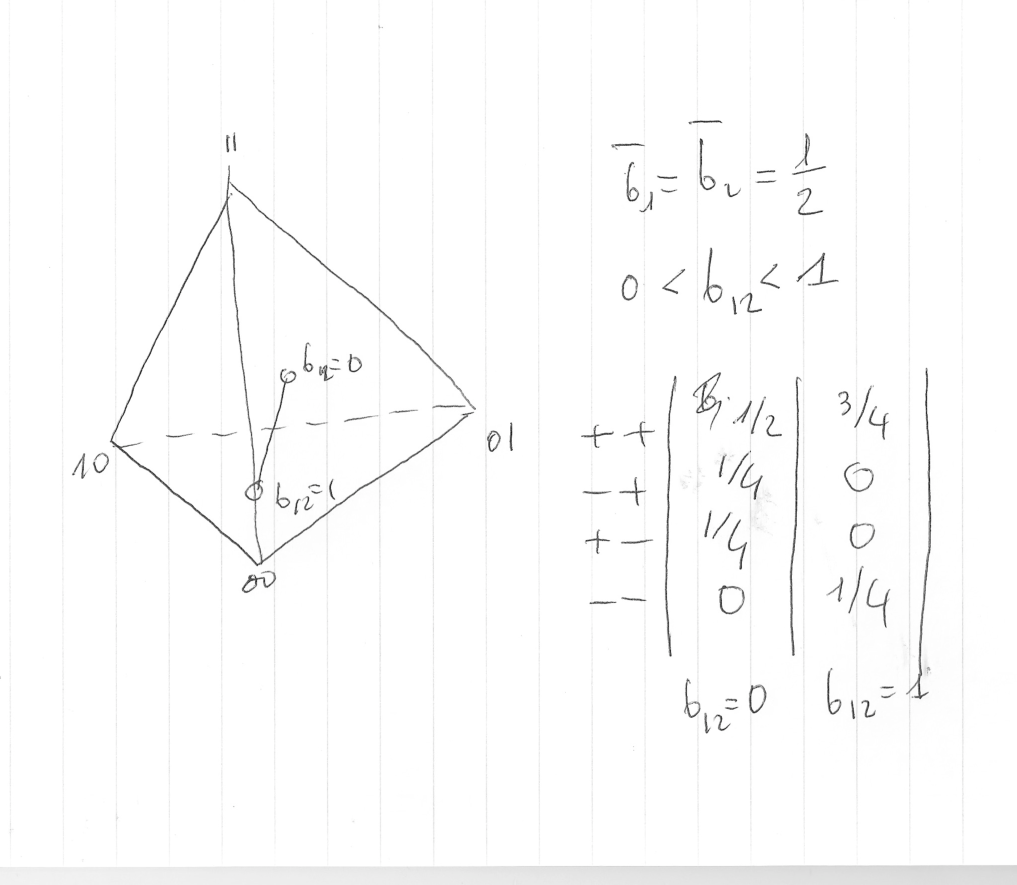
\includegraphics[width=.4\textwidth]{plan2x2.pdf}
    \caption{Plan on binary sample space}
    \label{fig:1}
  \end{figure}
%
We start with the case $n_1=n_2=2$. Let $\Omega_1=\Omega_2=\set{+,-}$, $\Omega=\set{++,+-,-+,--}$ Any function on $\Omega$ has the pseudo-Boolean form $f(x,y)=a_0+a_1 x + a_2 y + a_{12} xy$. In particular a probability has the form $\gamma(x,y) = \frac14(1+b_1x+b_2y+b_{12}xy)$ with $\gamma_1(x) = X_{\#}\gamma (x)= \frac12(1+b_1x)$, $\gamma_2(y) = Y_\# \gamma(y) = \frac12(1+b_2y)$. Given $\bar b_1, \bar b_2 \in ]-1,+1[$ to fix the margins, the plan is given by the 1 parameter family 
%
  \begin{equation*}
    \gamma(x,y) = \frac14(1+\bar b_1x+\bar b_2y+b_{12}xy), \quad -1 + \avalof{\bar b_1+\bar b_2} < b_{12} < 1 - \avalof{\bar b_1 - \bar b_2} \ .
  \end{equation*}
\end{exercise}

\subsection{Gradient flow}

\begin{proposition}Let be given a cost function $c \colon \Omega_1 \times \Omega_2 \to \reals$ and define the expected cost function $C \colon \SimO \ni \gamma \mapsto \expectat \gamma c$. Then the function $C$ restricted to the open plan $\Gamma^\circ(\mu_1,\mu_2)$ has statistical gradient
%
\begin{equation*}
 \grad_{\Gamma(\mu_1,\mu_2)} W \colon \gamma \mapsto w - \expectat \gamma w - w_{1,\gamma} - w_{2,\gamma} \in S_\gamma\Gamma(\mu_1,\mu_2) = (S_\gamma \oSimO)_{12} \ . 
\end{equation*}

It follows that the gradient flow of $W$ is
%
\begin{equation*}
  D\gamma(t) = - \left(w - \expectat \gamma w - w_{1,\gamma} - w_{2,\gamma}\right) \ .
\end{equation*}

Any solution $t \mapsto \gamma(t)$ of the gradient flow converges to a measure $\gamma* = \lim_{t \to \infty} \gamma(t) \in \SimO$ such that $\expectat {\gamma^*} w$ is the \emph{Gini dissimilarity} or \emph{Wasserstein distance} between $\mu_1$ and $\mu_2$,
%
\begin{equation*}
  \expectat {\gamma*} w = \min \setof{\expectat \gamma w}{ \gamma \in \Gamma(\mu_1,\mu_2)} \ .
\end{equation*}
%
 Moreover, the extension of the gradient to $\SimO$ is zero at $\gamma^*$, namely
%
\begin{equation*}
  w = \expectat {\gamma^*} w + w_{1,\gamma^*} + w_{2,\gamma^*}
\end{equation*}
%
on $\suppof{\gamma^*}$.
\end{proposition}

\begin{proof}
  
\end{proof}

\subsection{Kantorovich}

% \subsection{A Subsection Sample}
% Please note that the first paragraph of a section or subsection is
% not indented. The first paragraph that follows a table, figure,
% equation etc. does not need an indent, either.

% Subsequent paragraphs, however, are indented.

% \subsubsection{Sample Heading (Third Level)} Only two levels of
% headings should be numbered. Lower level headings remain unnumbered;
% they are formatted as run-in headings.

% \paragraph{Sample Heading (Fourth Level)}
% The contribution should contain no more than four levels of
% headings. Table~\ref{tab1} gives a summary of all heading levels.

% \begin{table}
% \caption{Table captions should be placed above the
% tables.}\label{tab1}
% \begin{tabular}{|l|l|l|}
% \hline
% Heading level &  Example & Font size and style\\
% \hline
% Title (centered) &  {\Large\bfseries Lecture Notes} & 14 point, bold\\
% 1st-level heading &  {\large\bfseries 1 Introduction} & 12 point, bold\\
% 2nd-level heading & {\bfseries 2.1 Printing Area} & 10 point, bold\\
% 3rd-level heading & {\bfseries Run-in Heading in Bold.} Text follows & 10 point, bold\\
% 4th-level heading & {\itshape Lowest Level Heading.} Text follows & 10 point, italic\\
% \hline
% \end{tabular}
% \end{table}


% \noindent Displayed equations are centered and set on a separate
% line.
% \begin{equation}
% x + y = z
% \end{equation}
% Please try to avoid rasterized images for line-art diagrams and
% schemas. Whenever possible, use vector graphics instead (see
% Fig.~\ref{fig1}).

% \begin{figure}
% \includegraphics[width=\textwidth]{fig1.eps}
% \caption{A figure caption is always placed below the illustration.
% Please note that short captions are centered, while long ones are
% justified by the macro package automatically.} \label{fig1}
% \end{figure}

% \begin{theorem}
% This is a sample theorem. The run-in heading is set in bold, while
% the following text appears in italics. Definitions, lemmas,
% propositions, and corollaries are styled the same way.
% \end{theorem}
% %
% % the environments 'definition', 'lemma', 'proposition', 'corollary',
% % 'remark', and 'example' are defined in the LLNCS documentclass as well.
% %
% \begin{proof}
% Proofs, examples, and remarks have the initial word in italics,
% while the following text appears in normal font.
% \end{proof}
% For citations of references, we prefer the use of square brackets
% and consecutive numbers. Citations using labels or the author/year
% convention are also acceptable. The following bibliography provides
% a sample reference list with entries for journal
% articles~\cite{ref_article1}, an LNCS chapter~\cite{ref_lncs1}, a
% book~\cite{ref_book1}, proceedings without editors~\cite{ref_proc1},
% and a homepage~\cite{ref_url1}. Multiple citations are grouped
% \cite{ref_article1,ref_lncs1,ref_book1},
% \cite{ref_article1,ref_book1,ref_proc1,ref_url1}.
%
% ---- Bibliography ----
%
% BibTeX users should specify bibliography style 'splncs04'.
% References will then be sorted and formatted in the correct style.
%
\bibliographystyle{splncs04}
\bibliography{tutto}
%
% \begin{thebibliography}{8}
% \bibitem{ref_article1}
% Author, F.: Article title. Journal \textbf{2}(5), 99--110 (2016)

% \bibitem{ref_lncs1}
% Author, F., Author, S.: Title of a proceedings paper. In: Editor,
% F., Editor, S. (eds.) CONFERENCE 2016, LNCS, vol. 9999, pp. 1--13.
% Springer, Heidelberg (2016). \doi{10.10007/1234567890}

% \bibitem{ref_book1}
% Author, F., Author, S., Author, T.: Book title. 2nd edn. Publisher,
% Location (1999)

% \bibitem{ref_proc1}
% Author, A.-B.: Contribution title. In: 9th International Proceedings
% on Proceedings, pp. 1--2. Publisher, Location (2010)

% \bibitem{ref_url1}
% LNCS Homepage, \url{http://www.springer.com/lncs}. Last accessed 4
% Oct 2017
% \end{thebibliography}
\end{document}
